\documentclass[tikz]{standalone}
\begin{document}
        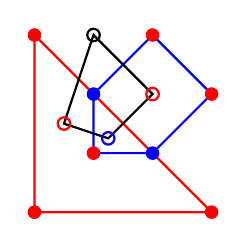
\begin{tikzpicture}[scale=0.75]
            \filldraw[red] (0,0) circle (3pt);
            \filldraw[red] (3,0) circle (3pt);
            \filldraw[red] (0,3) circle (3pt);
            \draw[red,thick] (0,0) -- (3,0) -- (0,3) -- cycle;
            
            \draw[blue,thick] (1,1) -- (2,1) -- (3,2) -- (2,3) -- (1,2) -- cycle;
            \filldraw[red] (1,1) circle (3pt);
            \filldraw[red] (3,2) circle (3pt);
            \filldraw[red] (2,3) circle (3pt);
            \filldraw[blue] (2,1) circle (3pt);
            \filldraw[blue] (1,2) circle (3pt);
            
            \draw[black,thick] (0.5,1.5) -- (1.25,1.25) -- (2,2) -- (1,3) -- cycle;
            \draw[red,thick] (0.5,1.5) circle (3pt);
            \draw[blue,thick] (1.25,1.25) circle (3pt);
            \draw[red,thick] (2,2) circle (3pt);
            \draw[black,thick] (1,3) circle (3pt);
        \end{tikzpicture}
\end{document}